\subsection{Projeto de Software}

A parte de software do projeto consiste essencialmente em reconhecer os comandos de voz feitos pelo usuário automaticamente, sem auxílio de palavras-chave ou de botões, recursos que costumam ser utilizados em outros projetos. Então o início do programa acontece ao identificar sinais no microfone em um volume mínimo pré-determinado. 
A partir desse instante o som começa a ser gravado, sendo que permanece desse modo durante alguns segundos. E após isso, o sinal de voz recebido será convertido para texto. Onde por fim, será analisado se as palavras recebidas têm correspondência com a lista de comandos pré-determinados. Caso tenham, será realizada a função equivalente ao comando. E caso contrário, indicará que ouve um erro e voltará para o início do programa.
O algoritmo correspondente à essa parte está apresentado na Figura \ref{fig-DiagramaSoftware} a seguir.

\begin{figure}[htbp]
	\centering
		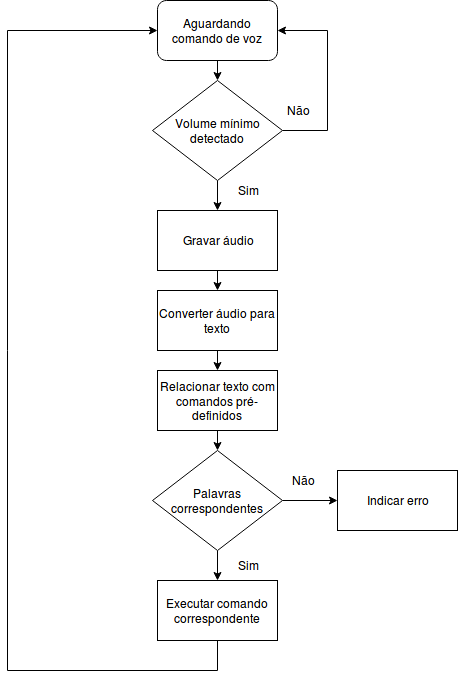
\includegraphics[scale=0.5]{DiagramaSoftware}
	\caption{Fluxograma do algoritmo}
	\label{fig-DiagramaSoftware}
\end{figure}
